
\setcounter{chapter}{2}
\chapter{Réalisation}
\minitoc %insert la minitoc
\graphicspath{{Chapitre3/figures/}}

%\DoPToC
%==============================================================================
\pagestyle{fancy}
\fancyhf{}
\fancyhead[R]{\bfseries\rightmark}
\fancyfoot[R]{\thepage}
\renewcommand{\headrulewidth}{0.5pt}
\renewcommand{\footrulewidth}{0pt}
\renewcommand{\chaptermark}[1]{\markboth{\MakeUppercase{\chaptername~\thechapter. #1 }}{}}
\renewcommand{\sectionmark}[1]{\markright{\thechapter.\thesection~ #1}}

\begin{spacing}{1.2}

%==============================================================================
\section*{Introduction}
Après  avoir  achevé  l’étape  de  conception  de  l’application,  on  va  entamer  dans  ce  chapitre  la  partie  réalisation  dans  laquelle  on  s’assure  que  le  système  est prêt pour être exploité par les utilisateurs finaux. A la fin de ce chapitre, les objectifs doivent avoir été atteints et le projet doit être clos.


\section{Diagramme de deploiment}

\begin{figure}[H]\centering
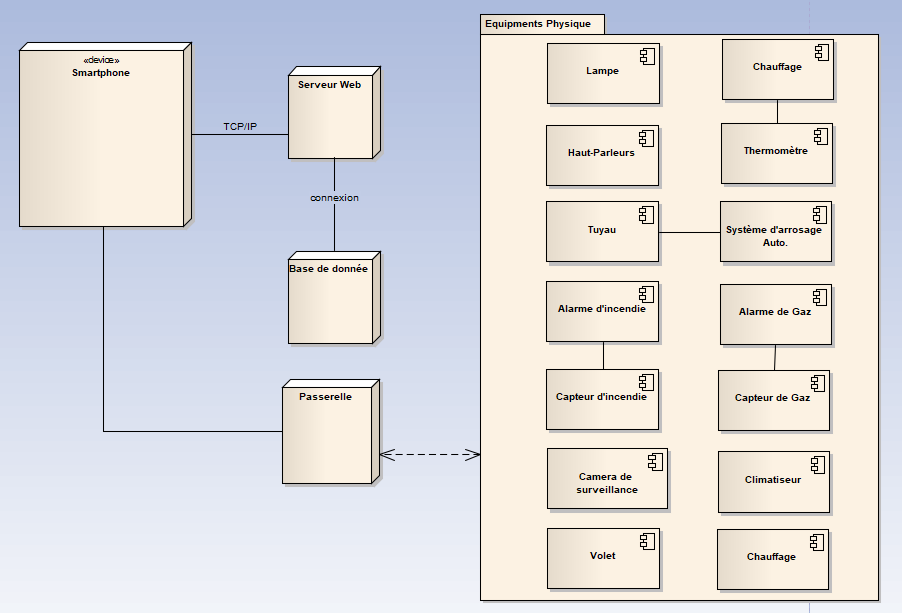
\includegraphics[scale=0.7]{33.png}
\caption{Diagramme de deploiment}
\label{fig:fig3}
\end{figure} 

\section{Outils et langages utilisés}
Pour la réalisation de ce projet, on a choisit d'utiliser le framework Javascript React Native développé par Facebook pour la  réalisation de l'application mobile multiplateforme, et le framwork Javascript React JS dévelopé aussi par Facebook pour la réalisation de l'interface web. \\
L'avantage majeur de ces deux frameworks , et plus précisément React Native, c'est qu'il est multiplateforme.
ce caractère est très important car il présente un besoins de notre projet. 

\newpage
\section{Présentation de l'application}
\subsection{Application Mobile}

\textbf{Page Accueil}
\begin{figure}[H]\centering
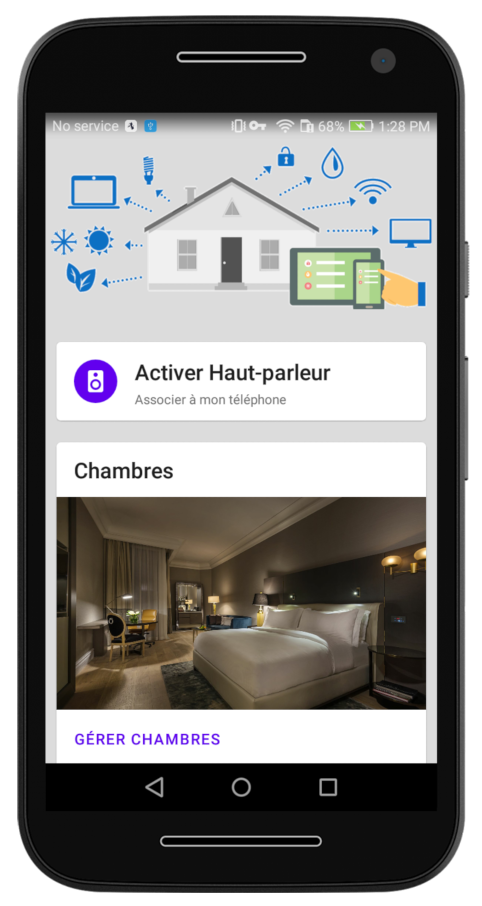
\includegraphics[scale=0.25]{1.png}
\caption{Application Mobile: Page Accueil}
\label{fig:fig3}
\end{figure} 

\textbf{Page Authentification par Code Pin}
\begin{figure}[H]\centering
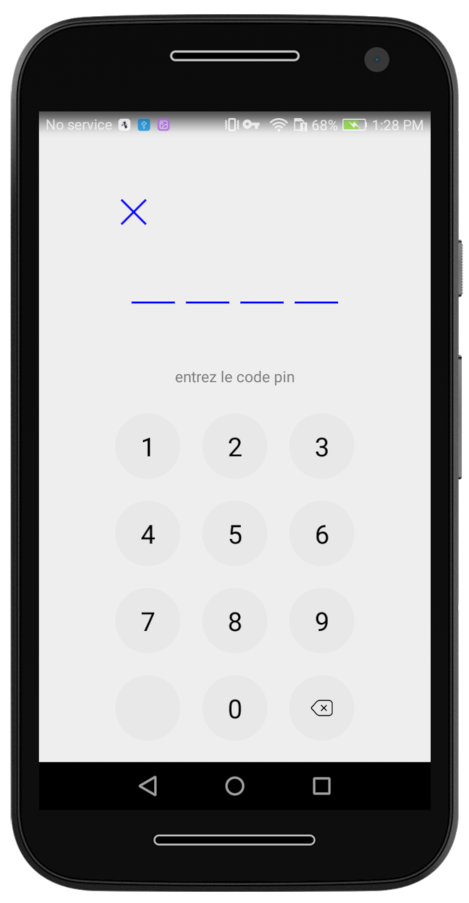
\includegraphics[scale=0.25]{2.png}
\caption{Application Mobile: Page Authentification par Code Pin}
\label{fig:fig3}
\end{figure} 

\textbf{Page Alarme}
\begin{figure}[H]\centering
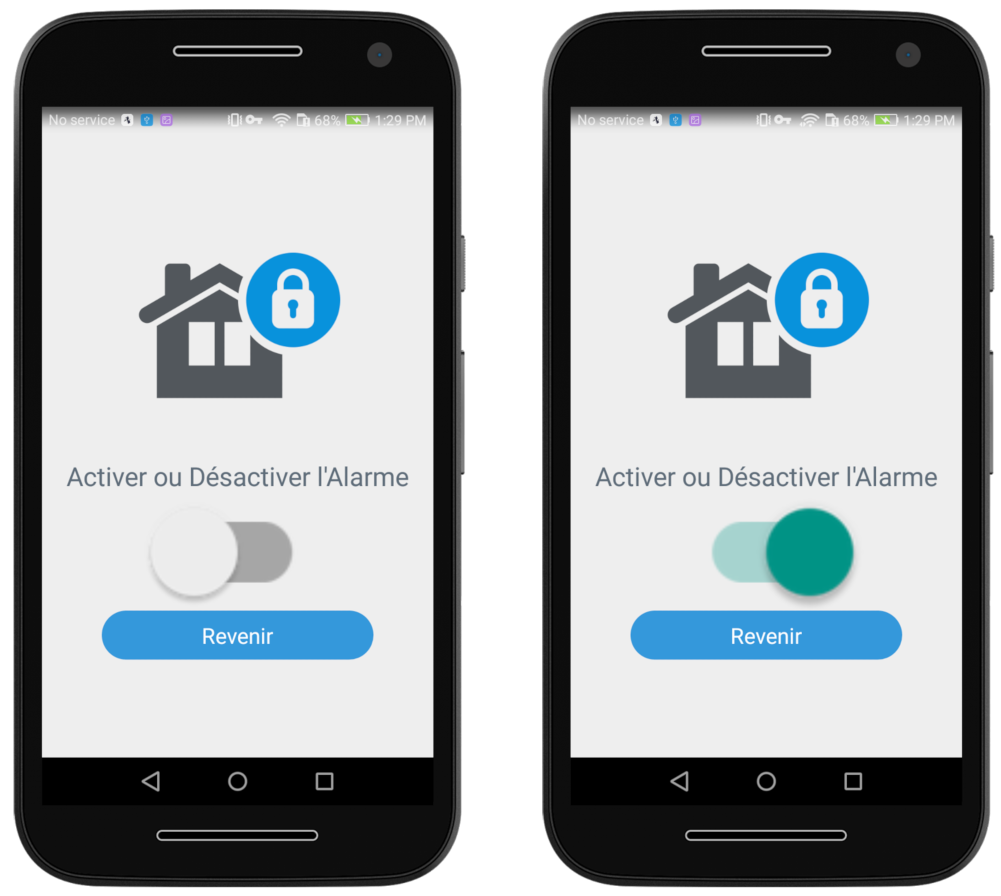
\includegraphics[scale=0.25]{3.png}
\caption{Application Mobile: Page Alarme}
\label{fig:fig3}
\end{figure} 

\subsection{Interface Web}

\begin{figure}[H]\centering
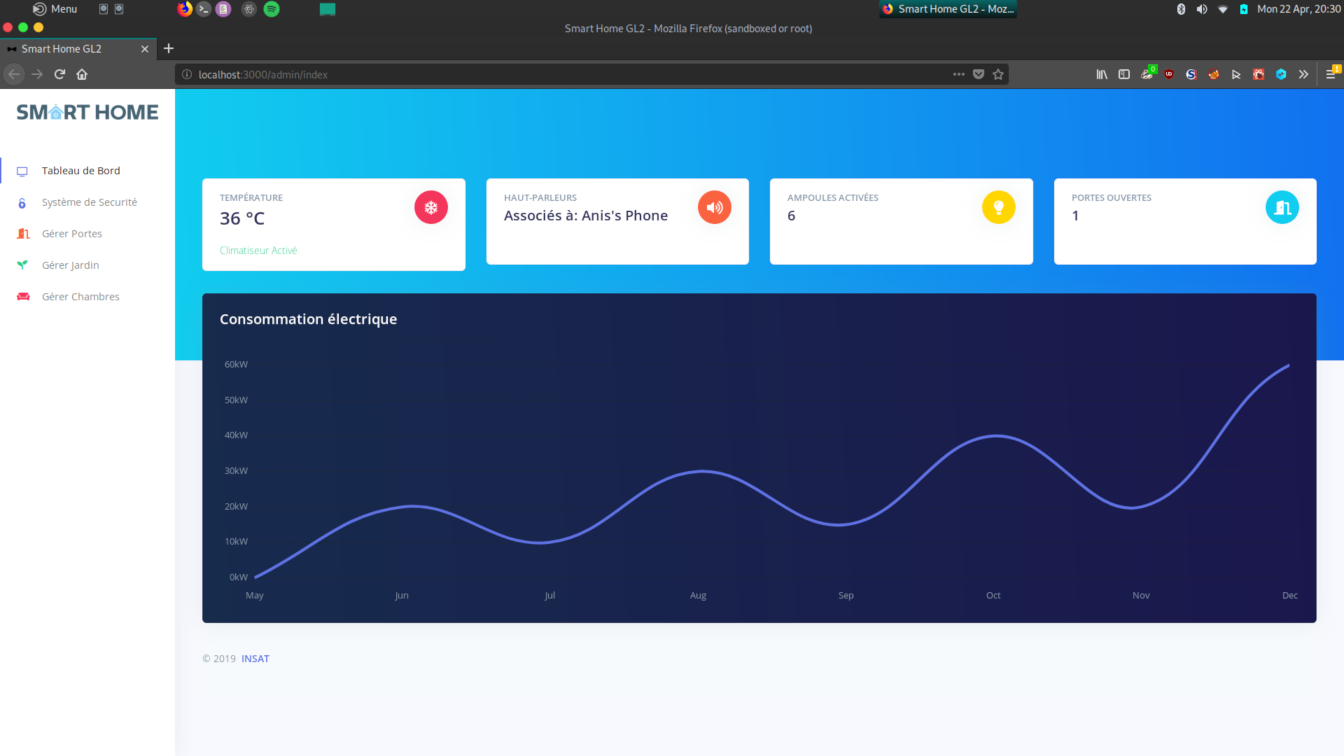
\includegraphics[scale=0.3]{4.png}
\caption{Interface Web: Page d'Accueil}
\label{fig:fig3}
\end{figure} 


\section*{Conclusion}
A travers ce chapitre, nous avons présenté la réalisation de l’application en justifiant nos choix technologiques, en représentant quelques interfaces graphiques que nous avons jugé les plus importantes.

%==============================================================================
\end{spacing}
